\documentclass[10pt, oneside]{article} 
\usepackage{amsmath, amsthm, amssymb, calrsfs, wasysym, verbatim, bbm, color, graphics, geometry, esint}
\usepackage{float}



\geometry{tmargin=.75in, bmargin=.75in, lmargin=.75in, rmargin = .75in}  

\newcommand{\bbR}{\mathbb{R}}
\newcommand{\bbC}{\mathbb{C}}
\newcommand{\bbZ}{\mathbb{Z}}
\newcommand{\bbN}{\mathbb{N}}
\newcommand{\bbQ}{\mathbb{Q}}
\newcommand{\Cdot}{\boldsymbol{\cdot}}
\newcommand{\scA}{\mathscr{A}}
\newcommand{\curl}{\text{curl}}

\theoremstyle{definition}
\newtheorem{exmp}{Example}[section]
\newtheorem{thm}{Theorem}
\newtheorem{defn}{Definition}
\newtheorem{prop}{Proposition}
\newtheorem{conv}{Convention}
\newtheorem{rem}{Remark}
\newtheorem{lem}{Lemma}
\newtheorem{cor}{Corollary}
% Copyright 2021 Paolo Adajar (padajar.com, paoloadajar@mit.edu)
% 
% Permission is hereby granted, free of charge, to any person obtaining a copy of this software and associated documentation files (the "Software"), to deal in the Software without restriction, including without limitation the rights to use, copy, modify, merge, publish, distribute, sublicense, and/or sell copies of the Software, and to permit persons to whom the Software is furnished to do so, subject to the following conditions:
%
% The above copyright notice and this permission notice shall be included in all copies or substantial portions of the Software.
% 
% THE SOFTWARE IS PROVIDED "AS IS", WITHOUT WARRANTY OF ANY KIND, EXPRESS OR IMPLIED, INCLUDING BUT NOT LIMITED TO THE WARRANTIES OF MERCHANTABILITY, FITNESS FOR A PARTICULAR PURPOSE AND NONINFRINGEMENT. IN NO EVENT SHALL THE AUTHORS OR COPYRIGHT HOLDERS BE LIABLE FOR ANY CLAIM, DAMAGES OR OTHER LIABILITY, WHETHER IN AN ACTION OF CONTRACT, TORT OR OTHERWISE, ARISING FROM, OUT OF OR IN CONNECTION WITH THE SOFTWARE OR THE USE OR OTHER DEALINGS IN THE SOFTWARE.

\usepackage{fullpage}
\usepackage{enumitem}
\usepackage{amsfonts, amssymb, amsmath,amsthm}
\usepackage{mathtools}
\usepackage[pdftex, pdfauthor={\name}, pdftitle={\classnum~\assignment}]{hyperref}
\usepackage[dvipsnames]{xcolor}
\usepackage{bbm}
\usepackage{graphicx}
\usepackage{mathrsfs}
\usepackage{pdfpages}
\usepackage{tabularx}
\usepackage{pdflscape}
\usepackage{makecell}
\usepackage{booktabs}
\usepackage{natbib}
\usepackage{caption}
\usepackage{subcaption}
\usepackage{physics}
\usepackage[many]{tcolorbox}
\usepackage{version}
\usepackage{ifthen}
\usepackage{cancel}
\usepackage{listings}
\usepackage{courier}

\usepackage{tikz}
\usepackage{istgame}

\hypersetup{
	colorlinks=true,
	linkcolor=blue,
	filecolor=magenta,
	urlcolor=blue,
}

\setlength{\parindent}{0mm}
\setlength{\parskip}{2mm}

\setlist[enumerate]{label=({\alph*})}
\setlist[enumerate, 2]{label=({\roman*})}

\allowdisplaybreaks[1]

\newcommand{\psetheader}{
	\ifthenelse{\isundefined{\collaborators}}{
		\begin{center}
			{\setlength{\parindent}{0cm} \setlength{\parskip}{0mm}
				
				{\textbf{\classnum~\semester:~\assignment} \hfill \name}
				
				\subject \hfill \href{mailto:\email}{\tt \email}
				
				Instructor(s):~\instructors \hfill Due Date:~\duedate	
				
				\hrulefill}
		\end{center}
	}{
		\begin{center}
			{\setlength{\parindent}{0cm} \setlength{\parskip}{0mm}
				
				{\textbf{\classnum~\semester:~\assignment} \hfill \name\footnote{Collaborator(s): \collaborators}}
				
				\subject \hfill \href{mailto:\email}{\tt \email}
				
				Instructor(s):~\instructors \hfill Due Date:~\duedate	
				
				\hrulefill}
		\end{center}
	}
}

\renewcommand{\thepage}{\classnum~\assignment \hfill \arabic{page}}

\makeatletter
\def\points{\@ifnextchar[{\@with}{\@without}}
\def\@with[#1]#2{{\ifthenelse{\equal{#2}{1}}{{[1 point, #1]}}{{[#2 points, #1]}}}}
\def\@without#1{\ifthenelse{\equal{#1}{1}}{{[1 point]}}{{[#1 points]}}}
\makeatother

\newtheoremstyle{theorem-custom}%
{}{}%
{}{}%
{\itshape}{.}%
{ }%
{\thmname{#1}\thmnumber{ #2}\thmnote{ (#3)}}

\theoremstyle{theorem-custom}

\newtheorem{theorem}{Theorem}
\newtheorem{lemma}[theorem]{Lemma}
\newtheorem{example}[theorem]{Example}

\newenvironment{problem}[1]{\color{black} #1}{}

\newenvironment{solution}{%
	\leavevmode\begin{tcolorbox}[breakable, colback=green!5!white,colframe=green!75!black, enhanced jigsaw] \proof[\scshape Solution:] \setlength{\parskip}{2mm}%
	}{\renewcommand{\qedsymbol}{$\blacksquare$} \endproof \end{tcolorbox}}

\newenvironment{reflection}{\begin{tcolorbox}[breakable, colback=black!8!white,colframe=black!60!white, enhanced jigsaw, parbox = false]\textsc{Reflections:}}{\end{tcolorbox}}

\newcommand{\qedh}{\renewcommand{\qedsymbol}{$\blacksquare$}\qedhere}

\definecolor{mygreen}{rgb}{0,0.6,0}
\definecolor{mygray}{rgb}{0.5,0.5,0.5}
\definecolor{mymauve}{rgb}{0.58,0,0.82}

% from https://github.com/satejsoman/stata-lstlisting
% language definition
\lstdefinelanguage{Stata}{
	% System commands
	morekeywords=[1]{regress, reg, summarize, sum, display, di, generate, gen, bysort, use, import, delimited, predict, quietly, probit, margins, test},
	% Reserved words
	morekeywords=[2]{aggregate, array, boolean, break, byte, case, catch, class, colvector, complex, const, continue, default, delegate, delete, do, double, else, eltypedef, end, enum, explicit, export, external, float, for, friend, function, global, goto, if, inline, int, local, long, mata, matrix, namespace, new, numeric, NULL, operator, orgtypedef, pointer, polymorphic, pragma, private, protected, public, quad, real, return, rowvector, scalar, short, signed, static, strL, string, struct, super, switch, template, this, throw, transmorphic, try, typedef, typename, union, unsigned, using, vector, version, virtual, void, volatile, while,},
	% Keywords
	morekeywords=[3]{forvalues, foreach, set},
	% Date and time functions
	morekeywords=[4]{bofd, Cdhms, Chms, Clock, clock, Cmdyhms, Cofc, cofC, Cofd, cofd, daily, date, day, dhms, dofb, dofC, dofc, dofh, dofm, dofq, dofw, dofy, dow, doy, halfyear, halfyearly, hh, hhC, hms, hofd, hours, mdy, mdyhms, minutes, mm, mmC, mofd, month, monthly, msofhours, msofminutes, msofseconds, qofd, quarter, quarterly, seconds, ss, ssC, tC, tc, td, th, tm, tq, tw, week, weekly, wofd, year, yearly, yh, ym, yofd, yq, yw,},
	% Mathematical functions
	morekeywords=[5]{abs, ceil, cloglog, comb, digamma, exp, expm1, floor, int, invcloglog, invlogit, ln, ln1m, ln, ln1p, ln, lnfactorial, lngamma, log, log10, log1m, log1p, logit, max, min, mod, reldif, round, sign, sqrt, sum, trigamma, trunc,},
	% Matrix functions
	morekeywords=[6]{cholesky, coleqnumb, colnfreeparms, colnumb, colsof, corr, det, diag, diag0cnt, el, get, hadamard, I, inv, invsym, issymmetric, J, matmissing, matuniform, mreldif, nullmat, roweqnumb, rownfreeparms, rownumb, rowsof, sweep, trace, vec, vecdiag, },
	% Programming functions
	morekeywords=[7]{autocode, byteorder, c, _caller, chop, abs, clip, cond, e, fileexists, fileread, filereaderror, filewrite, float, fmtwidth, has_eprop, inlist, inrange, irecode, matrix, maxbyte, maxdouble, maxfloat, maxint, maxlong, mi, minbyte, mindouble, minfloat, minint, minlong, missing, r, recode, replay, return, s, scalar, smallestdouble,},
	% Random-number functions
	morekeywords=[8]{rbeta, rbinomial, rcauchy, rchi2, rexponential, rgamma, rhypergeometric, rigaussian, rlaplace, rlogistic, rnbinomial, rnormal, rpoisson, rt, runiform, runiformint, rweibull, rweibullph,},
	% Selecting time-span functions
	morekeywords=[9]{tin, twithin,},
	% Statistical functions
	morekeywords=[10]{betaden, binomial, binomialp, binomialtail, binormal, cauchy, cauchyden, cauchytail, chi2, chi2den, chi2tail, dgammapda, dgammapdada, dgammapdadx, dgammapdx, dgammapdxdx, dunnettprob, exponential, exponentialden, exponentialtail, F, Fden, Ftail, gammaden, gammap, gammaptail, hypergeometric, hypergeometricp, ibeta, ibetatail, igaussian, igaussianden, igaussiantail, invbinomial, invbinomialtail, invcauchy, invcauchytail, invchi2, invchi2tail, invdunnettprob, invexponential, invexponentialtail, invF, invFtail, invgammap, invgammaptail, invibeta, invibetatail, invigaussian, invigaussiantail, invlaplace, invlaplacetail, invlogistic, invlogistictail, invnbinomial, invnbinomialtail, invnchi2, invnF, invnFtail, invnibeta, invnormal, invnt, invnttail, invpoisson, invpoissontail, invt, invttail, invtukeyprob, invweibull, invweibullph, invweibullphtail, invweibulltail, laplace, laplaceden, laplacetail, lncauchyden, lnigammaden, lnigaussianden, lniwishartden, lnlaplaceden, lnmvnormalden, lnnormal, lnnormalden, lnwishartden, logistic, logisticden, logistictail, nbetaden, nbinomial, nbinomialp, nbinomialtail, nchi2, nchi2den, nchi2tail, nF, nFden, nFtail, nibeta, normal, normalden, npnchi2, npnF, npnt, nt, ntden, nttail, poisson, poissonp, poissontail, t, tden, ttail, tukeyprob, weibull, weibullden, weibullph, weibullphden, weibullphtail, weibulltail,},
	% String functions 
	morekeywords=[11]{abbrev, char, collatorlocale, collatorversion, indexnot, plural, plural, real, regexm, regexr, regexs, soundex, soundex_nara, strcat, strdup, string, strofreal, string, strofreal, stritrim, strlen, strlower, strltrim, strmatch, strofreal, strofreal, strpos, strproper, strreverse, strrpos, strrtrim, strtoname, strtrim, strupper, subinstr, subinword, substr, tobytes, uchar, udstrlen, udsubstr, uisdigit, uisletter, ustrcompare, ustrcompareex, ustrfix, ustrfrom, ustrinvalidcnt, ustrleft, ustrlen, ustrlower, ustrltrim, ustrnormalize, ustrpos, ustrregexm, ustrregexra, ustrregexrf, ustrregexs, ustrreverse, ustrright, ustrrpos, ustrrtrim, ustrsortkey, ustrsortkeyex, ustrtitle, ustrto, ustrtohex, ustrtoname, ustrtrim, ustrunescape, ustrupper, ustrword, ustrwordcount, usubinstr, usubstr, word, wordbreaklocale, worcount,},
	% Trig functions
	morekeywords=[12]{acos, acosh, asin, asinh, atan, atanh, cos, cosh, sin, sinh, tan, tanh,},
	morecomment=[l]{//},
	% morecomment=[l]{*},  // `*` maybe used as multiply operator. So use `//` as line comment.
	morecomment=[s]{/*}{*/},
	% The following is used by macros, like `lags'.
	morestring=[b]{`}{'},
	% morestring=[d]{'},
	morestring=[b]",
	morestring=[d]",
	% morestring=[d]{\\`},
	% morestring=[b]{'},
	sensitive=true,
}

\lstset{ 
	backgroundcolor=\color{white},   % choose the background color; you must add \usepackage{color} or \usepackage{xcolor}; should come as last argument
	basicstyle=\footnotesize\ttfamily,        % the size of the fonts that are used for the code
	breakatwhitespace=false,         % sets if automatic breaks should only happen at whitespace
	breaklines=true,                 % sets automatic line breaking
	captionpos=b,                    % sets the caption-position to bottom
	commentstyle=\color{mygreen},    % comment style
	deletekeywords={...},            % if you want to delete keywords from the given language
	escapeinside={\%*}{*)},          % if you want to add LaTeX within your code
	extendedchars=true,              % lets you use non-ASCII characters; for 8-bits encodings only, does not work with UTF-8
	firstnumber=0,                % start line enumeration with line 1000
	frame=single,	                   % adds a frame around the code
	keepspaces=true,                 % keeps spaces in text, useful for keeping indentation of code (possibly needs columns=flexible)
	keywordstyle=\color{blue},       % keyword style
	language=Octave,                 % the language of the code
	morekeywords={*,...},            % if you want to add more keywords to the set
	numbers=left,                    % where to put the line-numbers; possible values are (none, left, right)
	numbersep=5pt,                   % how far the line-numbers are from the code
	numberstyle=\tiny\color{mygray}, % the style that is used for the line-numbers
	rulecolor=\color{black},         % if not set, the frame-color may be changed on line-breaks within not-black text (e.g. comments (green here))
	showspaces=false,                % show spaces everywhere adding particular underscores; it overrides 'showstringspaces'
	showstringspaces=false,          % underline spaces within strings only
	showtabs=false,                  % show tabs within strings adding particular underscores
	stepnumber=2,                    % the step between two line-numbers. If it's 1, each line will be numbered
	stringstyle=\color{mymauve},     % string literal style
	tabsize=2,	                   % sets default tabsize to 2 spaces
%	title=\lstname,                   % show the filename of files included with \lstinputlisting; also try caption instead of title
	xleftmargin=0.25cm
}



\title{UChicago SSI: Formal Theory: 13210}
\author{Notes by Agustín Esteva, Lectures by Scott Gehlbach}
\date{Academic Year 2024-2025}

\begin{document}

\maketitle
\tableofcontents

\vspace{.25in}

\section{Lectures}

\subsection{Monday, Jan 6: Interactions}
Solutions to making people behave themselves:
\begin{enumerate}
    \item \textbf{Sacrifice:} voluntary individual sacrifice for others.
    \begin{itemize}
        \item \textit{Example of people not taking wallets with money (except in Mexico)}
    \end{itemize}
    \item \textbf{Cooperation:} coordinating actions for mutual benefit.
    \begin{itemize}
        \item \textit{Example of firms}
    \end{itemize}
    \item \textbf{Coercion:} individuals forced to take actions which will benefit others.
    \begin{itemize}
        \item \textit{Example of laws (driving)}
    \end{itemize}
\end{enumerate}
\textbf{Differences in outcomes are driven by differences in institutions}
\begin{def}
    An institution is defined to be the "rules of the game.``
\end{def}
\begin{rem}
    We can think of them as constitutions and laws, or as conventions and customs. Acemoglu/Robinson argue that political institutions influence economic institutions which influence economic growth.
\end{rem}

\subsection{Wednesday, Jan 8}
\begin{defn}
    We say a person is \textit{selfish} when she lacks kindness toward and responsibility for others.
\end{defn}
\begin{defn}
    We say a person is \textit{rational} if she takes actions that are consistent with her goals.
\end{defn}
\begin{rem}
    We say a person is \textit{irrational} if they are not rational. There are three main types:
    \begin{enumerate}
        \item To forget or neglect goals (drunk before a test)
        \item To draw wrong conclusions from the information at hand (classic human errors)
        \item To hold incorrect beliefs for other reasons (Coronavirus beliefs)
    \end{enumerate}
\end{rem}
\begin{defn}
    \textit{Expected utility theory} describes the decision-maker's preferences through a utility function and the beliefs through a probability function. The action with the highest expected utility is then chosen by the decision maker.
\end{defn}

\begin{defn}
(Under certainty)
    Given a set of alternatives $X$ and a preference relation $R$ on $X,$ we define the \textit{utility function} $u(x)$ represents $R$ if and only if, for all $x,y \in X,$ $u(x) \geq u(y)$ if and only if $xRy.$
\end{defn}
\begin{rem}
    If $u(\cdot)$ is a utility representing $R$ on $X,$ then 
    \[M(R, X) = \arg\max_{x\in U}u(x)\]
\end{rem}


\begin{defn}
    We represent \textit{utility functions} in generality with the following form
    \begin{align}
    \textbf{u}_i (\textbf{s}) = U_i(c(s)) + \lambda_i v(s),    
    \end{align}
     where $\textbf{s} = (s_1, \dots, s_n)$ denotes the actions that relevant people take, $c = (c_1, \dots, c_n)$ denotes the consumption of the $n$ people that $u$ cares about, $U_i$ denotes person $i's$ utility, $\lambda_i$ denotes the extent to which $i$ cares about social values, $v$ denotes the social values.
\end{defn}
\begin{rem}
    \textit{Economics is about individual's choices, sociology is about how individuals don't have any choices to make.} When $\lambda \to \infty,$ the individual follows society, or a \textit{logic of appropriateness.} When $\lambda = 0,$ individuals follow a \textit{logic of consequences.}
\end{rem}
\begin{rem}
    When a person is selfish, a persons utility and goals coincide with their own consumption, and we denoted this by saying that if $i$ is selfish, then
    \[u_i(s) = U_i(s_i(s))\]
\end{rem}

\begin{thm}
    Under certain conditions, there exists a function $u$ that assigns a number $u_j$ for each outcome $x_j$ such that the expected utility of a lottery $\textbf{p}_j = (p_{i1}, \dots, p_{in})$ induced by action $i$ is given by 
    \[U(\textbf{p}_i) = \sum_{j=1}^n p_{ij} uj\] and $\textbf{p}_i R \textbf{p}_k$ if and only if $U(\textbf{p}_i)\geq U(\textbf{p}_k).$
\end{thm}

\begin{defn}
    When a person's action has an impact on somebody else's utility, we say the action causes an \textit{externality.}
\end{defn}
We can impose a positive, negative, or neutral externality to other people.
\begin{defn}
    An outcome (a strategy profile $s$ or a consequence $c$) is said to be efficient if there does not exist another outcome that yields higher utility (that is better for some and worse for none).
\end{defn}
\newpage
\subsection{Monday, Jan 13: Situations, Games, and Cooperation}
\begin{defn}
    A \textit{social situation} (or a \textit{game form}) comprises of three elements:
    \begin{enumerate}
        \item The people involved in the situation (the \textit{players})
        \item The information and actions that are available to them (the \textit{strategies})
        \item The potential results of those actions (the \textit{consequences})
    \end{enumerate}
\end{defn}
\begin{defn}
    A \textit{game} is a game form together with a utility function for each player.
\end{defn}
\begin{figure}[H]
    \centering
    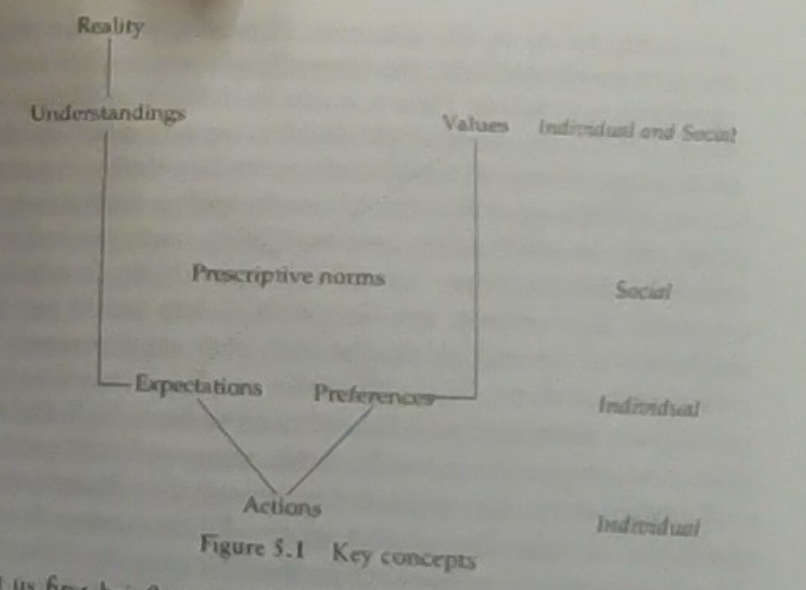
\includegraphics[width=0.5\linewidth]{Images/The Group and the Individual.png}
    \caption{The Group and the Individual}
\end{figure}





\newpage
\subsection{Wednesday, Jan 15: Nash Equilibrium}
\begin{defn}
    A \textbf{strategic game} is defined by:
    \begin{enumerate}
        \item Players: $i\in [n].$
        \item Actions: An action is an element $a_i \in A_i$ where $A_i$ is player $i'$s \textbf{action space} and an \textbf{action profile} is defined to be $a = (a_1, \dots, a_N)\in A.$ Some more notation, $a_{-i}$ denotes the action profile for all players other than player $i.$ I.e, $a_{-i}= (a_1, \dots, a_{i-1}, a_{i+1}, \dots, a_N).$
        \item Preferences: preferences over action profiles are typically represented in utility form. 
    \end{enumerate}
\end{defn}

\begin{rem}
    In Ellingsen, a game form is a social situation that includes the players, the strategies/actions, and the consequences. A game is a game form and the preferences. I.e, a game includes the utility functions necessary for the calculations later on. Consider the following Prisioner's dilemna, where person A can either sacrifice (-1 dollar to A, +2 dollars to B) or not (-0 dollars to A, +0 dollars to B), and B can do the same. This is a game form in Table 1.
    \begin{table}[H]
        \centering
        \begin{tabular}{c|c|c}
             & S & N\\
             \hline
             S& (2,2) & (0,3) \\
             \hline
             N&  (3,0)& (1,1)\\
        \end{tabular}
        \caption{Bilateral Sacrifice Situation (Consequences)}
    \end{table}
    Now consider selfish players with utility function $U_i = c_i,$ this is now a game!
    \begin{table}[H]
        \centering
        \begin{tabular}{c|c|c}
             & S & N\\
             \hline
             S& (2,2) & (0,3) \\
             \hline
             N&  (3,0)& (1,1)\\
        \end{tabular}
        \caption{Bilateral Sacrifice Game (Selfish Utility)}
    \end{table}
    Consider now another game of altruistic players with $\alpha$ level of altruisim\footnote{Recall that the utility function of an altruistic player is $U_i = c_i  + \alpha c_j$}:
    \begin{table}[H]
        \centering
        \begin{tabular}{c|c|c}
             & S & N\\
             \hline
             S& (2 + 2\alpha,2 + 2\alpha) & (3\alpha,3) \\
             \hline
             N&  (3\alpha,3)& (1 + \alpha,1 + \alpha)\\
        \end{tabular}
        \caption{Bilateral Sacrifice Game (Altruistic Utility)}
    \end{table}
    Finally consider when both players are egalitarian\footnote{Recall that the utility function of an egalitarian player is $U_i = c_i - \beta|c_i - c_j|$}:
    \begin{table}[H]
        \centering
        \begin{tabular}{c|c|c}
             & S & N\\
             \hline
             S& (2,2) & (-3\beta, 3- 3\beta) \\
             \hline
             N&  (3 - 3\beta,-3\beta)& (1,1)\\
        \end{tabular}
        \caption{Bilateral Sacrifice Game (Egalitarian Utility)}
    \end{table}
\end{rem}
\begin{defn}
    We say an action $a_i''$ \textbf{strictly dominates} $a_i'$ if and only if for all $a_{-i},$ we have that 
    \[u_i(a_i'', a_{-i}) > u_i(a_i', a_{-i})\]
\end{defn}
\begin{rem}
    In Table 2, $N$ strictly dominates $S$ for every player.
\end{rem}
Consider the battle of the sexes:
 \begin{table}[H]
        \centering
        \begin{tabular}{c|c|c}
             & Opera & Boxing\\
             \hline
             Opera& (2,1) & (0,0) \\
             \hline
             Boxing&  (0,0)& (1,2)\\
        \end{tabular}
        \caption{The Battle of the Sexes}
    \end{table}
In words, Nash equilibrium is everybody doing the best they can given what other people are doing:
\begin{defn}
    An action profile $a^\ast \in A$ is a \textbf{Nash equilibrium} if and only if 
    \[u_i(a^\ast)\geq u_i(a_i, a_{-i}^\ast)\] for all $a_i \in A_i$ for each player $i.$
\end{defn}
\begin{rem}
    Nash equilibrium corresponds to a steady state of the game, it embodies a stable social norm. No individual has any reason to deviate from it!
\end{rem}
Thus, in the battle of the sexes, $a^\ast \in \{(\text{Opera-Opera)}, \text{(Boxing-Boxing})\}$ is a Nash equilibrium.\\
Why is it reasonable? Why are the player's beliefs about other's actions reasonable?
\begin{enumerate}
    \item Repeated play
    \item Mediator
    \item Communication
    \item Focal point
\end{enumerate}
\begin{defn}
    We define a \textbf{best response} to be a set valued function such that 
    \[B_i(a_{-i}) = \{a_i \in A_i : u_i(a_i, a_{i-1}) \geq u_i(a_i', a_{-i}) \quad \forall \; a_i' \in A_i\}.\]
\end{defn}
\begin{rem}
    In the battle of the sexes, we have that 
    \[B_1(\text{Box}) = \text{Box}, \quad B_1(\text{Opera}) = \text{Opera}\]
\end{rem}


\begin{prop}
    An action profile $a^\ast \in A$ is a Nash equilibrium if and only if $a_i^\ast \in B_i(a_{i-1})$ for all $i \in [n].$
\end{prop}

\begin{defn}
    An outcome is a \textbf{Pareto efficient} outcome if there is no other outcome such that every actor is at least as well of and at least one actor that is strictly better off. That is, if an outcome is PE, then moving to any other outcome results in players getting worse than before.
\end{defn}
\begin{rem}
    Nash equilibrium does not imply Pareto efficient (consider Table 2's equilibria of $(1,1)$.)
\end{rem}
\begin{defn}
    A group engages in voluntary \textbf{cooperation} if each member of the group takes an action that benefits others (given what they do), even though that action is not certain to benefit oneself.
\end{defn}

\newpage
\subsection{Wednesday, Jan 22: Models of Anarchy}
Hobbes, ever the optimist, describes in \textit{Leviathan} in 1651 his views on anarchy (Part I, Ch. 13, Para 9):
\begin{quote}
    \dots wherein men live without other security, that what their own strength, and their own invention shall furnish them withall,\dots and the life of a man, solitary, poor, nasty, brutish, and short.
\end{quote}
Thus, man cannot truly live without governance. Can we model this? Well I can't but Ellingsen can. Let there be two individuals, $i$ and $j,$ who can divide their labor-time (normalized to $1$) between making food ($x_i$) and making weapons ($y_i$):
\[y_i = 1- x_i.\] The total food production is $x_1 + x_2 = x$ and the total weapons production is $y_1 + y_2 = y.$ Both $i$ and $j$ are selfish\footnote{Recall that the utility function of a selfish player is $U_i = c_1$} and $c_1 + c_2 = x$ since people cannot eat weapons\footnote{Evidently Ellingsen is not American} and all the food will be eaten. $x_{\max} = 2$ when $y = 0$ and vice versa:
\begin{figure}[H]
    \centering
    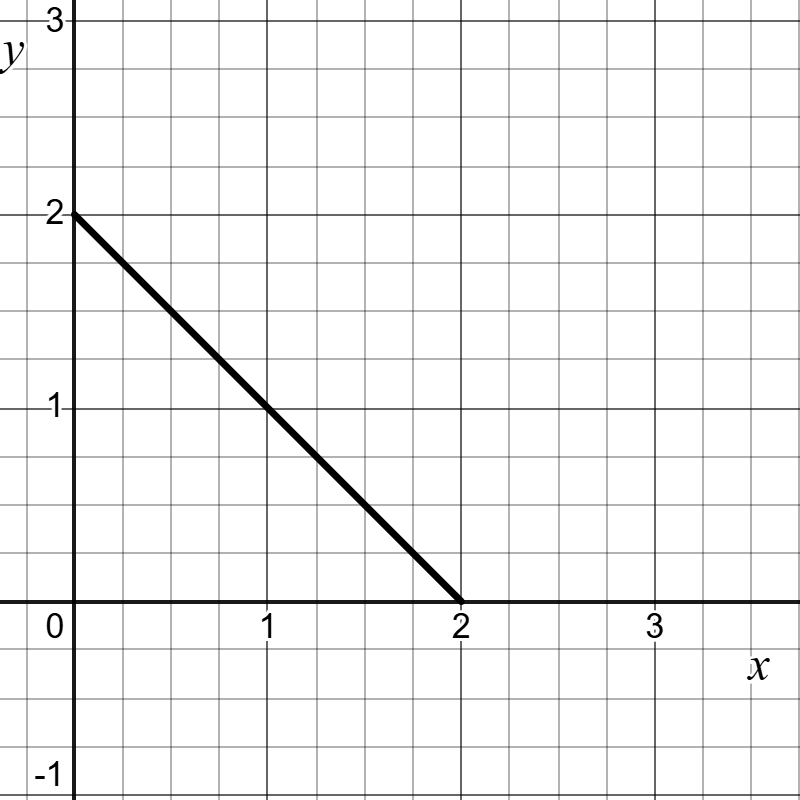
\includegraphics[width=0.25\linewidth]{Images/Production_Possibilities.png}
    \caption{Production Possibilities}
\end{figure}
\begin{figure}[H]
    \centering
    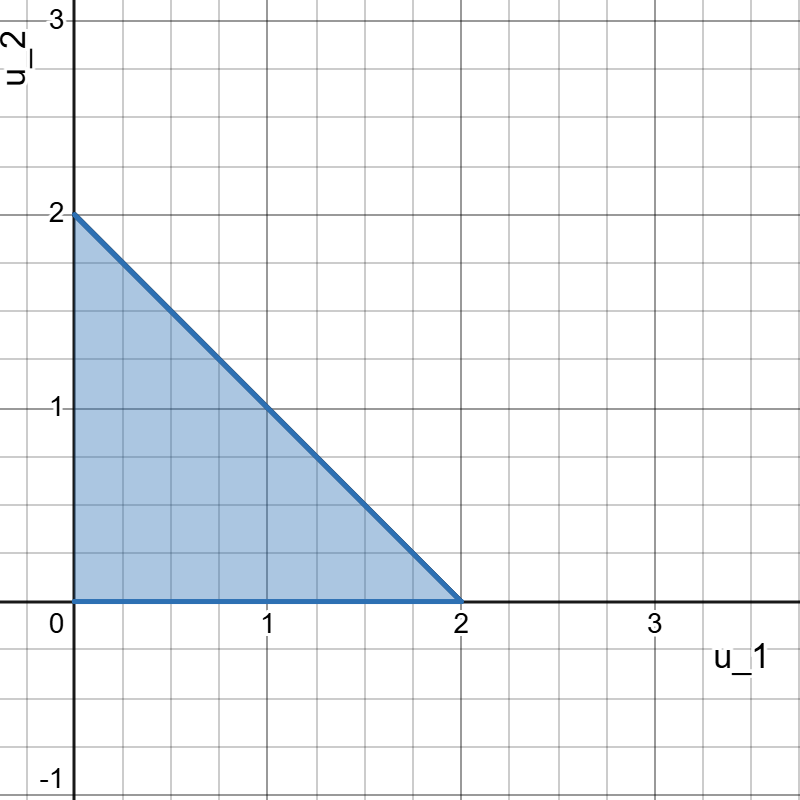
\includegraphics[width=0.25\linewidth]{Images/Consumption_Possibilities.png}
    \caption{Consumption Possibilities}
\end{figure}
By Hobbes, the only thing that matters is strength, and thus the person with the most weapons gets all the food:

\[u_i(y_i, y_j) = \begin{cases}
    x, \qquad y_i > y_j\\
    \frac{x}{2}, \qquad y_i = y_j\\
    0, \qquad y_i < y_j
\end{cases}\]
Thus, the only Nash equilibrium is $y_1 = y_2 = 1.$ Everybody spends all their time making weapons\dots
\begin{rem}
    How do we fix this? Hobbes argued for a leviathan (a king/strong ruler with the power to control the people). Rousseau argues that humans are not governed by the selfish natured we imposed on them, and that we would need to establish a social contract in order for the few to not only benefit the few. Montesquieu argued that this government should be split in order to check and balance itself.\footnote{Of course, both Rousseau and Montesquieu are French, so take them with a grain of salt. Hobbes is english, so ignore him. Listen to Tommy Jefferson.}
\end{rem}

Consider the following game:
\begin{table}[H]
        \centering
        \begin{tabular}{c|c|c}
             & S & N\\
             \hline
             S& (2,2) & (0, 3) \\
             \hline
             N&  (3,0)& (1,1)\\
        \end{tabular}
        \caption{Pareto vs Nash}
    \end{table}
Here, we have that $(N,N)$ is the Nash Equilibrium, but all the other outcomes are Pareto Efficient. Now lets consider this next game with rule compliance:
\begin{table}[H]
        \centering
        \begin{tabular}{c|c|c}
             & S & N\\
             \hline
             S& (2,2) & (0, 3 - \lambda\mu) \\
             \hline
             N&  (3 - \lambda\mu,0)& (1 - \lambda\mu,1 - \lambda\mu)\\
        \end{tabular}
        \caption{Nash Equilibrium with Rule Compliance}
    \end{table}
Intuitively, when $\lambda\mu$ gets really large, the cost of not sacrificing grows immense. Thus, $(S,S)$ is a Nash equilibrium when $\lambda\mu \geq 1.$ If the inequality is an equality, then everything is an equilbria...
\begin{table}[H]
        \centering
        \begin{tabular}{c|c|c}
             & S & N\\
             \hline
             S& (2 + 2\alpha,2 + 2\alpha) & (3\alpha, 3) \\
             \hline
             N&  (3, 3\alpha)& (1 + \alpha,1 +  \alpha)\\
        \end{tabular}
        \caption{Nash Equilibrium with Altruism}
    \end{table}
The Nash Equilibrium will change when $(2 + 2\alpha)\geq 3 \implies \alpha \geq \frac{1}{2},$ which is the tipping point. If more than the only $(S,S).$ If equality, then all. If strictly less than, then only $(N,N).$

\begin{table}[H]
        \centering
        \begin{tabular}{c|c|c}
             & S & N\\
             \hline
             S& (2,2 ) & (-3\beta, 3 - 3\beta) \\
             \hline
             N&  (3 - 3\beta, -3\beta)& (1,1)\\
        \end{tabular}
        \caption{Nash Equilibrium with Egalitarianism}
    \end{table}
Tipping points of $2\geq 3 - 3\beta \implies 1\leq 3\beta \implies \beta \geq \frac{1}{3}$ and $-3\beta \geq 1 \implies \beta \geq \frac{-1}{3}.$
\begin{exmp}
    Consider the game where two players choose $x_1,x_2 \in [0,100]$ and in which the player who chooses the closest to half of the mean wins. Players prefer winning to tying to losing.
    
    (Existence) Consider the action profile $(0,0).$ Then suppose WLOG that $x_1$ deviates to some $x>0.$ Then since $\frac{x}{4}$ is closer to $0$ than to $x,$ player $2$ wins and thus both players choosing $0$ is a Nash Equilibrium.

    (Uniqueness) Let $(x_1, x_2)$ be the numbers chosen by the two players. Then the player closest to $\frac{x_1 + x_2}{4}$ will win. If $x_2 < x_1,$ then $x_2$ is closer to the required quantity.
\end{exmp}
\begin{exmp}
(Cournot Model) 
\begin{itemize}
    \item Two firms, $i = 1,2$
    \item Each firm chooses a quantity $q_i \in \bbR^+$
    \item Firms prefer more profit to less
    \item Profit:
    \[\pi_i = pq_i - cq_i = q_i(p-c),\] where $c$ is the marginal cost of production and price $P$ is determined by the inverse demand function
    \[p = \max[\alpha - q_1- q_2, 0],\] where $\alpha>c.$
\end{itemize}
Looking at best response function:
\[b_1 = \arg\max_{q_1} \pi_1 = \max_{q_1} q_1(\alpha - q_1 - q_2 - c).\] is a convex function, and thus taking the derivative and setting equal to $0,$ we get that 
\[q_1(q_2) = \frac{\alpha - c - q_2}{2}\] is the best response for player $1.$ Symmetrically
\[q_2(q_1) = \frac{\alpha - c - q_1}{2}\] is the best response for player $2.$ Best responses coincide at 
\[q_1 = \frac{\alpha - c}{3}, \qquad q_2  = \frac{\alpha - c}{3}.\]
\end{exmp}
\newpage

\subsection{Monday, Jan 27: The Leviathan}
Assume the presence of a (nonstrategic) state (the leviathan) that imposes a cost $\gamma >1$ if any player $i$ that chooses $y_i >0.$ Let players $1,2$ be in the Ellingsen-Hobbes scenario, but now
\[u_i = c_i - \gamma\mathbf{1}_{y_i > 0},\] then the Nash Equilibrium is $y_1 = y_2 = 1.$


\newpage
\subsection{Wednesday, Jan 29: The Tragedy of the Commons}
Two players, $i = 1,2,$ and each player extracts $c_i \in [0,y]$ in period $1,$ where $y>0$ us a stock of a common-property resource. There is a second period they also worry about:
\[u_i(c_1, c_2) = \ln(c_i) + \ln\left(\frac{y - c_1 - c_2}{2}\right).\] Note that everything will be consumed by the end of period 2. Finding the Nash Equilibrium with the best response method, we must first find the best response of player $1$ from the consumption of player $2$ as $c_2.$ Maximizizng the utility function $u_1:$
\[0 = \frac{1}{c_1} - \frac{1}{y - c_1 - c_2} \implies b_1(c_2) = \frac{y-c_2}{2}\] By symmetry, 
\[b_2(c_1) = \frac{y-c_1}{2}\]
Thus, we get that setting them equal to each other, we find that the Nash Equilibrium is uniquely defined by:
\[(c_1^\ast, c_2^\ast) = (\frac{y}{3}, \frac{y}{3}).\] Thus, the equilibrium utility is 
\[u(c_1^\ast, c_2^\ast) = \ln(\frac{y}{3}) + \ln(\frac{y}{6}),\] and thus the commons are overgrazed. Comparing this to the social optimum of 
\[\max_{c_1, c_2}\left[\ln(c_1) + \ln(c_2) + 2\ln\left(\frac{y - c_1 - c_2}{2}\right)\right] \implies (c_1^W, c_2^W) = (\frac{y}{4}, \frac{y}{4}).\] How do we solve this issue?
\begin{enumerate}
    \item privatization of the commons: Each player will receive $\frac{y}{2}$ of the commons:
    \[u_1(c_1) = \ln(c_1) + \ln\left(\frac{y}{2} - c_1\right) \implies c_1^\ast = \frac{y}{4}\] and equally, 
    \[c_2^\ast = \frac{y}{4}\]
\end{enumerate}

\begin{quote}
    If men were angels, no government would be necessary. If angels were to govern men, neither external nor internal controls on government would be necessary.
\end{quote}
\tab -Federalist 51

\newpage
\subsection*{Monday, Feb 3: Coordination Games}

Rousseau's Stag Hunt:
    \begin{table}[H]
        \centering
        \begin{tabular}{c|c|c}
             & S & H\\
             \hline
             S& (9,9) & (0,8) \\
             \hline
             H&  (8,0)& (7,7)\\
        \end{tabular}
        \caption{Stag Hunt}
    \end{table}
The weak link has a massive effect on performance. Solutions to coordination problems:
\begin{enumerate}
    \item Sending a costless message to the other players \textit{might help} 
    \item Have a boss (manager)
\end{enumerate}
\begin{defn}
    A message is \textit{self committing} if the sender wants to do whatever the message entailed if the receiver believed the message.
\end{defn}
\begin{defn}
    A message is \textit{self-signaling} if the sender intends to do what she says.
\end{defn}
When is coordination not desirable? The game of chicken:
\begin{table}[H]
        \centering
        \begin{tabular}{c|c|c}
             & H & D\\
             \hline
             H& (0,0) & (4,1) \\
             \hline
             D&  (1,4)& (3,3)\\
        \end{tabular}
        \caption{Chicken!}
    \end{table}
Common Knowledge Problem:\begin{table}[H]
        \centering
        \begin{tabular}{c|c|c}
             & Stay & Leave\\
             \hline
             Stay& (1,1) & (0,0) \\
             \hline
             Leave&  (0,0)& (2,2)\\
        \end{tabular}
        \caption{Should I Stay or Should I Go?}
    \end{table}
The above problem is solved with common knowledge. Creating Common Knowledge:
\begin{enumerate}
    \item Ads
    \item Meetings
    \item cc:
    \item Rituals
\end{enumerate}

\newpage
\subsection*{Wednesday, Feb 5: Midterm}
\begin{enumerate}
    \item Consider an elaboration of a two players, two actions coordination game in which, prior to play of the game, one player can send a costless message stating which of the two actions she intends to play. Such an action is necessarily:
    \begin{enumerate}
        \item Self-signaling but not self-committing.
        \item Self-committing but not self-signaling.
        \item Both self-signaling and self-committing.
        \item Neither self-signaling nor self-committing.
    \end{enumerate}
    \textbf{Solution: b.}
    \item The idea athat women with young children should stay at home is an exmaple of a 
    One the one hand, two are stirctly dominant, but not pareto efficient
\end{enumerate}


\newpage
\subsection*{Monday, Feb 10: Mixed Strategy Games}
Schelling: Coordination is more imagination than rationality.





\newpage
\subsection*{Wednesday: Feb 13: Mixed-Strategy Games}
\begin{defn}
    A \textbf{strategic game with vNM preferences} is defined by 
    \begin{enumerate}
        \item Players
        \item Actions
        \item Preferences over lotteries over action profiles that may be represented by an expected payoff function.
    \end{enumerate}
    \end{defn}

    \begin{defn}
        A \textbf{mixed strategy} is a probability distribution over actions.
    \end{defn}
    \begin{defn}
        A \textbf{pure strategy} is a mixed strategy that assigns probability $1$ to some action.
    \end{defn}
    \begin{defn}
        A mixed strategy profile, $\alpha^*,$ is a \textbf{mixed-strategy Nash equilibrium} if and only if 
        \[U_i(\alpha^*) \geq U_i(\alpha_i, \alpha_{-i}^*), \qquad \forall \;\alpha_i, \; \forall\; i \in [n].\]
    \end{defn}
    \begin{table}[H]
        \centering
        \begin{tabular}{c|c|c}
             & Left & Right\\
             \hline
             Left& (1,-1) & (-1,1) \\
             \hline
             Right&  (-1,1)& (1,-1)\\
        \end{tabular}
        \caption{Penalties with von Neumann}
    \end{table}
    Suppose player $1$ believes player $2$ will play $L$ with probability $q$ and thus $R$ with probability $(1-q).$ Thus:
    \[u_1(L, q) = q(1) + (1-q)(-1) = 2q - 1\]
    \[u_1(R, q) = q(-1) + (1-q)(1)= 1-2q\]
    Plotting these gives:
    \begin{figure}[H]
        \centering
        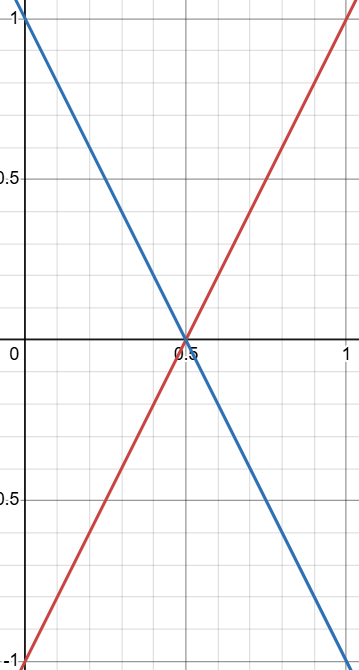
\includegraphics[width=0.10\linewidth]{Images/Matching Pennies.png}
        \caption{Red is $u_1(L),$ blue is $u_1(R)$}
    \end{figure}
    Thus, we see that $u_1(L) = u_1(R)$ when $q = \frac{1}{2}.$ If $q< \frac{1}{2},$ then player 1's first response is to go right, and so $p = 1$ and thus player $1$ has a pure strategy of $R.$ If $q>\frac{1}{2},$ then player $1$ wants to play $L$ and thus $p = 1.$ Thus, the best response function of player $1$ is given by:
    \begin{figure}[H]
        \centering
        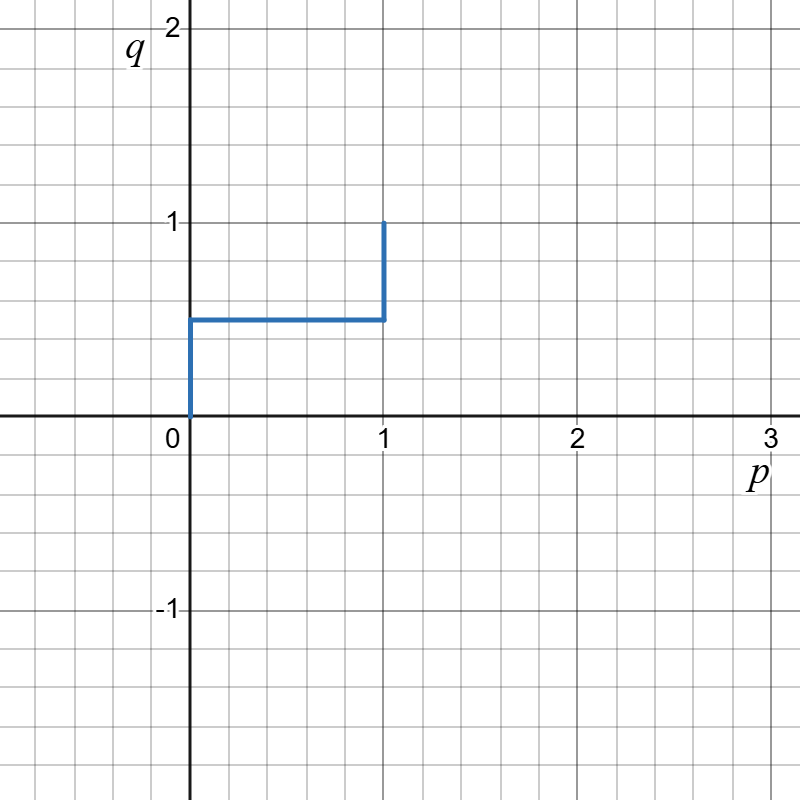
\includegraphics[width=0.25\linewidth]{Images/BRPMP.png}
        \caption{Best Response of player $1$}
    \end{figure}
    Symmetrically, we find that the black graph is player $2$s best response function:
    \begin{figure}[H]
        \centering
        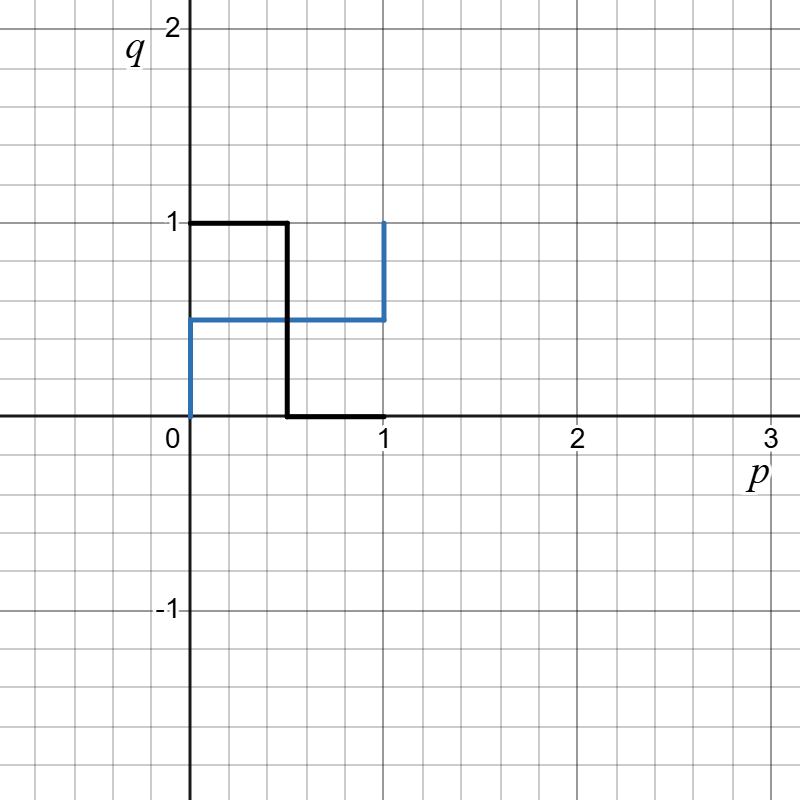
\includegraphics[width=0.25\linewidth]{Images/Notanazi.png}
        \caption{Best Response functions}
    \end{figure}
    Thus, we find that $(p^*, q^*) = (\frac{1}{2}, \frac{1}{2})$ or equivalently, $\left((\frac{1}{2}L, \frac{1}{2}R), (\frac{1}{2}L, \frac{1}{2}R)\right).$
\begin{thm}
    Every strategic game with vNM preferences in which each player has finitely many actions has a mixed-strategy Nash equilibrium.
\end{thm}
\begin{exmp}
    \begin{table}[H]
        \centering
        \begin{tabular}{c|c|c}
             & O & B\\
             \hline
             O& (2,1) & (0,0) \\
             \hline
             B&  (0,0)& (1,2)\\
        \end{tabular}
        \caption{BoS with von Neumann}
    \end{table}
    \[u_1(O) = 2q, \qquad u_1(B) = 1-q \implies q' = \frac{1}{3}, u_1(O) = u_1(B)\]
    \[u_2(O) = p, \qquad u_2(B) = 2(1-p) \implies p' = \frac{2p}{3}, u_2(O) = u_2(B)\] Plotting the best response functions:
     And thus 
\begin{figure}[H]
        \centering
        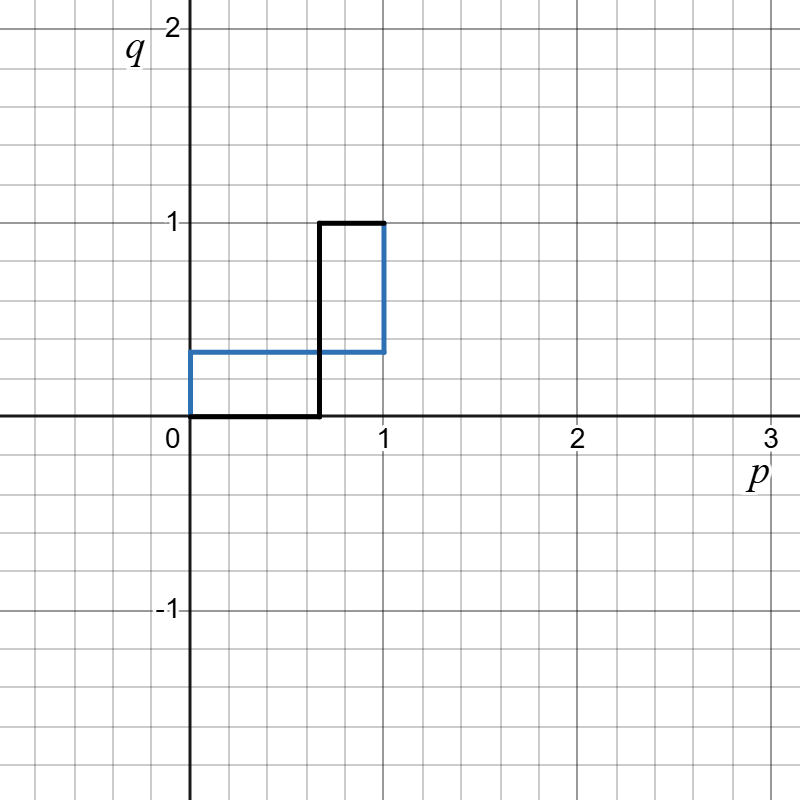
\includegraphics[width=0.5\linewidth]{Images/BoSvNM.png}
        \caption{BoS Best Response Functions}
    \end{figure}
        \[(p^*, q^*)  = \{(\frac{2}{3}, \frac{1}{3}), (0,0), (1,1)\}\]
\end{exmp}

\newpage
\subsection{Monday, Feb 17: Extensive Games}

\begin{defn}
    An \textbf{extensive game with perfect information} is defined by:
    \begin{enumerate}
        \item Players
        \item Terminal Histories:
        \begin{itemize}
            \item \textit{sub history:} For some sequence of actions $(a^{1}, a^{2}, \dots, a^k),$ a sequence of actions, $(a^{1}, a^{2}, \dots, a^m)$ with $m\in [k]$ or the empty history.
            \begin{itemize}
                \item A \textit{proper sub history} is a sub history such that $m<k$ or the empty history
            \end{itemize}
            \item A \textit{terminal history} is a sequence of actions that is not a proper sub history of any other sequence.
            \item A \textit{history} is a sub history of some terminal history.
        \end{itemize}
        \item Player function, which signs a player for every proper sub history of some terminal history
        \item Preferences over terminal histories.
    \end{enumerate}
\end{defn}

\begin{exmp}
    Prisoner's Dilemma:
    Players: 1,2
    Terminal Histories: $(C,C), (C,D), (D, C), (D,D)$
    Player function: $P(\emptyset) = 1, P(C) = 2, P(D) = 2$
    Preferences: Obvious from picture
\end{exmp}
\begin{defn}
    The \textbf{action space} for player assigned to history $h$ is 
    \[A(h):= \{a \; : \; (h,a) \text{ is a history}\}\]
\end{defn}
\begin{exmp}
    In our example, $A(\emptyset) = \{C, D\}.$
\end{exmp}
\begin{defn}
    A \textbf{strategy} $s_i$ for player $i$ assigns an action in $A(h)$ at each history $h$ assigned to $i$ (a complete contingent plan)
\end{defn}
\begin{exmp}
    $s_1(A(\emptyset)) = \{C,D\}$

    
    $s_2(A(C)) = \{CC, CD\}$ or $s_2(A(D)) = \{DC, DD\}$  and so $s_2(A(h)) = \{CC, CD, DC, DD\}$
\end{exmp}

\begin{defn}
    The \textbf{outcome} of $s,$ $O(s),$ is the terminal history if each player $i$ players $s_i.$
\end{defn}
\begin{exmp}
    Suppose $s = (C,CD),$ then $O(s) = (C,C)$

    Suppose $S = (D,DC),$ then $O(s)  = (D,C)$
\end{exmp}

\begin{rem}
    In multistage games where a player plays more than once, think of the doofus friend when coming up with all the strategies, and so you need to have a strategy which has an action at \textit{every} history where each player has a choice to make.
\end{rem}
\begin{defn}
    A strategy profile $s^*$ is a Nash equilibrium if and only if
    \[u_i(O(s^*)) \geq u_i(O(s_i, s^*_{-i})), \qquad \forall s_i, \forall i\]
\end{defn}
\begin{exmp}
    To find the Nash equilibrium of the multi-stage P.D. game above, we can write down the strategic form of the game:
    \begin{table}[H]
        \centering
        \begin{tabular}{c|c|c | c | c}
             & CC & CD & DC & DD\\
             \hline
             C& (2,2) & (2^*,2) & (0,3^*)& (0,3^*)\\
             \hline
             D&  (3^*,0)& (1,1^*) & (3^*,0) & (1^*,1^*)\\
        \end{tabular}
        \caption{Multi-Stage P.D. Strategic Form}
    \end{table}
\end{exmp}

For sub-game perfect Nash equilibrium, start at the end of the game, find optimal action, and prune the suboptimal actions and repeat. 


\newpage
\subsection{Wednesday, Feb 19: Bargaining Games}
\begin{defn}
    A strategy profile $s^*$  is a \textbf{subgame-perfect Nash equilibrium} if and only if in no subgame can any player $i$ do better by choosing a strategy different from $s_i^*$ given that every other player $j$ adheres to $s_j^*.$
\end{defn}
\begin{rem}
    Note that SPNE are Nash Equilibrium.
\end{rem}hi

\begin{exmp}
    (Ultimatum Bargaining Game)
    \begin{itemize}
        \item Player $1$ makes an offerer of:
        \[x = (x_1, x_2), \quad x_i = \text{share of pie for player $i$}\]
        \[x_i, x_2 \in [0,1]\]
        \[x_1 + x_2 = 1\]
        \item Player $2$ can accept or reject, if player $2$ rejects, they both receive $0.$
        \item Player's preferences represented by share of pie they receive.
    \end{itemize}
    \begin{figure} [H]
        \centering
        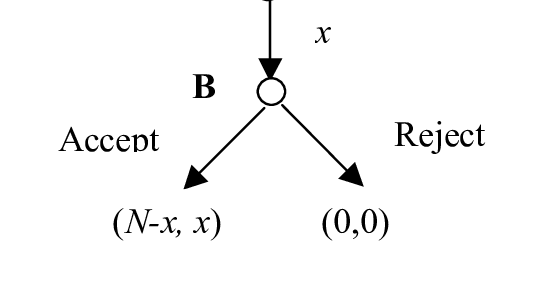
\includegraphics[width=0.5\linewidth]{Images/UBG.png}
        \caption{Ultimatum Bargaining Game in Extended Form, where $N=1$ and $x$ is $x_1.$}
    \end{figure}
    Obviously, it is a best response for player $2$ to accept if $x_2 >0.$ If $x_2 = 0,$ then they are both best responses. Thus, Nash equilibrium is $(1,0).$ where $P2$ accepts if $x_2 >0$ and accepts if $x_2 = 0.$
\end{exmp}

\newpage
\subsection*{Monday, Feb 24: Repeated Game}
\begin{defn}
    A \textbf{stage game} $G$ is a strategic game with actions $a_i \ni A_i$ and payoff function $u_i$ for each player $i.$
\end{defn}
\begin{defn}
    A \textbf{repeated game} $G(T, \delta)$ is a stage game $G$ for $T$ periods where $T \in (0, \infty] \cap \bbN.$ At each period $t,$ each player chooses $a_i \in A_i$ having observed the full history. Preferences over terminal histories $(a^1, a^2, \dots)$ given by 
    \[\sum_{t = 1}^T \delta^{t-1}u_i(a^t)\] where $a^t$ is the action profile played in period $t$ and $\delta \in (0,1).$
\end{defn}
\begin{exmp}
Play this game twice:
    \begin{table}[H]
        \centering
        \begin{tabular}{c|c|c}
             & C & D\\
             \hline
             C& (6,6) & (-1,8) \\
             \hline
             D&  (8,-1)& (1,1)\\
        \end{tabular}
        \caption{Finite Prisoner's Dilemma}
    \end{table}
    There are 5 different subgames (one subgame per outcome of first game and the entire game)

To find SPNE, we solve by backwards induction. For each subgame in period $2,$ the Nash Equilibrium is $(D,D).$ Thus, in the first period, we have that if $\delta$ is the discount factor, then 
    \begin{table}[H]
        \centering
        \begin{tabular}{c|c|c}
             & C & D\\
             \hline
             C& (6 + \delta,6 + \delta) & (-1+ \delta,8+ \delta) \\
             \hline
             D&  (8+ \delta,-1+ \delta)& (1+ \delta,1+ \delta)\\
        \end{tabular}
        \caption{Finite Prisoner's Dilemma, Backward's Induction}
    \end{table}
    And so period $1$ is $(D,D).$ Thus, 
    \[s_1* = (D, D | O(s^1) \in \{ (C,C), (C,D), (D,C), (D,D)\}), \qquad s_2^* = (D, D) | O(s^1) \in \{ (C,C), (C,D), (D,C), (D,D)\}\]
\end{exmp}

\begin{exmp}
    \begin{table}[H]
        \centering
        \begin{tabular}{c|c|c | c}
             & C & D & E\\
             \hline
             C& (6,6 ) & (-1,8) & (1,7) \\
             \hline
             D&  (8,-1)& (\textbf{1,1}) & (4,0)\\
             \hline
             E & (7,1) & (0,4) & (\textbf{4,4})
        \end{tabular}
        \caption{Finitely Repeated Modified PD}
    \end{table}
    Suppose we play Table 18 twice. At time $2,$ NE are $(D,D)$ and $(E,E).$ Thus, SPNE:
    \[s_i = \begin{cases}
        C, \qquad t = 1\\
        E\qquad t = 2 | (C,C) @t = 1,\\
        D, \qquad \text{else}
    \end{cases}\] since 
    the `temptation'  is $7-6$ and the punishment is $(4 - 1)\delta.$ Thus, in order for the players to coordinate, we need $3\delta \geq 1 \implies \delta\geq \frac{1}{3}.$
\end{exmp}
Suppose now Table 16 (classic PD) is repeated infinitely. Then if both players coordinate every period, we will have that 
\[u_1 = 6 + 6\delta+ 6\delta^2 + \dots = 6\sum_{t=0}^\infty \delta^t = \frac{6}{1-\delta}\]

\begin{defn}
    The \textbf{one deviation property} states that no player can increase her payoff by changing her action at the start of any subgame in which she is the first mover, given the other player's strategies and the rest of her own strategy.
\end{defn}

\begin{prop}
    A strategy profile is a SPNE if and only if it satisfies the one-deviation property.
\end{prop}

\newpage
\subsection*{Wednesday, Feb 26: Infinitely Repeated Prisoner's Dilemma}
\begin{defn}
    In an infinitely repeating prisioner's dillema, a \textbf{grim trigger} strategy is for each player $i,$
    \[s_i = \begin{cases}
        C, \qquad \forall t \text{ if always $(C,C)$ previously}\\
        D, \qquad t>t_0 \text{ Where at $t_0$ something other than $(C,C)$ was played}
    \end{cases}\]
\end{defn}
\begin{rem}
    In state-transition represenation, we have that 
    \[\boxed{\underline{C}: C}\xrightarrow[]{(D,C), (C,D),(D,D)} \boxed{\underline{D}: D},\] where the right box is self absorbing (can't leave). We need to check SPNE in both states:
    \begin{itemize}
        \item ($\underline{D}$) Both players today recieve:
        \[u_i= \sum_{i=1}^\infty \delta^i = \frac{1}{1-\delta}\] For a player to not deviate, we need to have that the player should not benefit from switching to cooperating in this period, and thus
        \[\frac{1}{1-\delta} \geq -1  + \delta + \delta^2 + \dots,\] which is true. Thus, the one deviation property is met and so $\underline{D}$ is an SPNE.
        \item ($\underline{C}$) Both players recieve:
        \[u_i = 6 + 6\delta + \dots = \frac{6}{1-\delta}\] If a player deviates, then they recieve 
        \[u_i' = 8 + 1\delta + \delta^2 + \dots = 8 + \frac{\delta}{1-\delta}\] Thus, we must have that 
        \[6 \geq 8(1-\delta) + \delta \iff \delta \geq \frac{2}{7}\]
    \end{itemize}
\end{rem}

\begin{exmp}
Consider the following infinitely repeated prisoner's dilemma:
    \begin{table}[H]
        \centering
        \begin{tabular}{c|c|c}
             & C & D\\
             \hline
             C& (6,6) & (-1,8) \\
             \hline
             D&  (8,-1)& (1,1)\\
        \end{tabular}
        \caption{Infinite Prisoner's Dilemma}
    \end{table}
To see that 
\[\boxed{\underline{C}: C}\xrightarrow[]{(D,C), (C,D),(D,D)} \boxed{\underline{D}: D},\] the state transitions are SPNE, we must have that
    \begin{itemize}
        \item $(\underline{D}):$ In the current state, we have that both players recieve
        \[u_i = 0 + 0 + \dots = 0.\] If they defect, then 
        \[u_i = -1 + 0 + \dots.\] Thus, not defecting is optimal since $0\geq -1.$
        \item $(\underline{C})$  In the current state, we have that both players recieve
        \[u_i = 3 + 3\delta + \dots = \frac{3}{1-\delta}\] If they defect then 
        \[u_i' = 7  + 0 + \dots = 7.\] Thus, we must have that in order for $\underline{C}$ to be an SPNE, then 
        \[\frac{3}{1-\delta} \geq 7 \iff 3 \geq 7 - 7\delta \implies \delta \geq \frac{4}{7},\] which is always true. 
    \end{itemize}
\end{exmp}

\begin{defn}
    The \textbf{discounted average payoff} is 
    \[\overline{u}_\delta = (1-\delta)\sum_{t=1}^\infty \delta^{t-1}w_t\]
\end{defn}
\begin{exmp}
    Suppose that in the prevoius example, the players oscillate bewteen periods by changing from $(C,C)$ to $(D,D),$ then 
    \[u_i = 3 + 0\delta + 3\delta^2 + \dots = \frac{3}{1-\delta^2}.\] Thus, we have that 
    \[\overline{u_\delta} = \frac{3}{1-\delta^2}(1-\delta) = \frac{3}{(1 + \delta)(1-\delta)}(1-\delta) = \frac{3}{1+ \delta}\]
\end{exmp}

\begin{defn}
    The \textbf{feasible payoffs} are all the weighted averages payoffs profiles in a strategic game.
\end{defn}
\begin{exmp}
    
\begin{figure}[H]
    \centering
    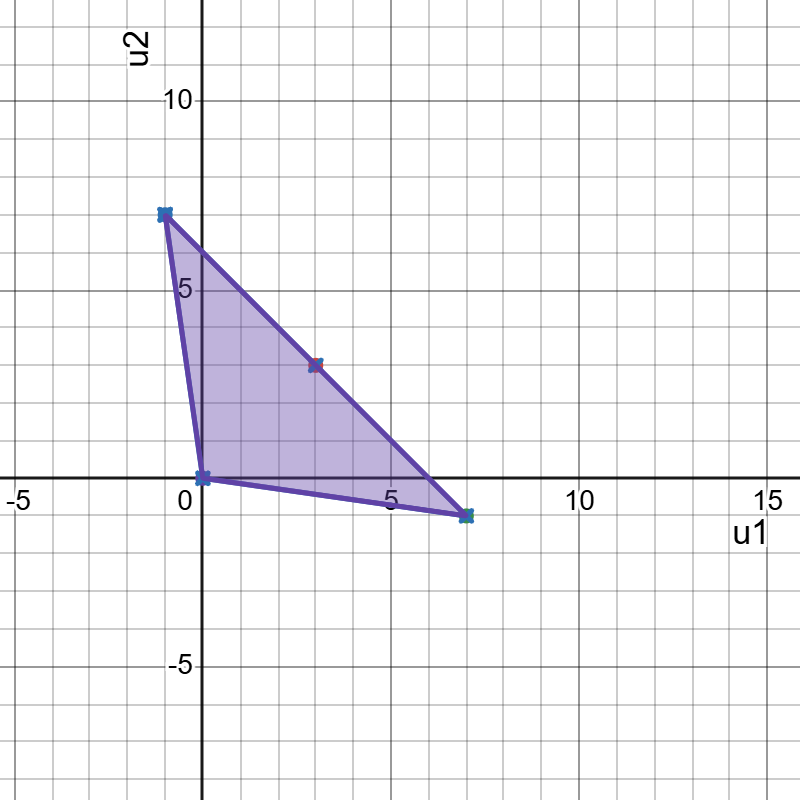
\includegraphics[width=0.5\linewidth]{SSI 1/Exmp.png}
    \caption{Feasible Payoffs}
\end{figure}
\end{exmp}

\begin{thm}
    (Folk Theorem) Let $(x_1, x_2)$ be a pair of feasible payoffs in the stage game $G$ for which $x_i$ is greater than the worst payoff player $i$ can receive in a Nash equilibrium of $G$. Then there exists $\overline{\delta} < 1$ such that if $\delta>\overline{\delta},$ the infinitely repeated game $G$ has SPNE in which the discounted average payoff of each player $i$ is $x_i.$
\end{thm}
\begin{proof}
    The proof is constructive.
\end{proof}

Ostrom's Design Principles for Self-Governance
\begin{enumerate}
    \item Clearly defined boundaries
    \item Congruence tween rules and local conditions
    \item Collective-choice arrangements
    \item Local monitoring
    \item Graduated sanctions
    \item Conflict-resolution dilemmas
    \item Minimal recognition of right to organize
    \item Nested enterprises
\end{enumerate}

\begin{defn}
    \begin{enumerate}
        \item \textbf{First-level dilemma} Incentives to underinvest, overfish $,\dots,$ can be solved through self-governance. But!
        \item \textbf{second-level dilemma} institutions themselves are public goods, and thus have an incentive to underinvest.
    \end{enumerate}
\end{defn}

\newpage
\subsection{Monday, March 3: Enforcers}
11- Pick, 1- Keller
\begin{table}[H]
        \centering
        \begin{tabular}{c | c}
             & \\
             \hline
             S& (0,3) \\
             \hline
             NS&(1,0)\\
        \end{tabular}
        \caption{Rowena (First Stage)}
    \end{table}
\begin{table}[H]
        \centering
        \begin{tabular}{c | c|  c}
             & R & NR\\
             \hline
             & (2,0) & (0,2) \\
        \end{tabular}
        \caption{Colin (Second Stage)}
    \end{table}
\begin{table}[H]
        \centering
        \begin{tabular}{c| c}
              \\
             \hline
             P& (-\rho,\pi) \\
             \hline
             NP&(0,0)\\
        \end{tabular}
        \caption{Rowena (Third Stage)}
    \end{table}
Suppose the game is played only once, then using backwards induction to find SPNE:
\begin{enumerate}
    \item Stage 3: NP $(0\geq -\rho)$
    \item Stage 2: NR $(2 \geq 0)$
    \item Stage 3: NS $(1 \geq 0)$
\end{enumerate}
Strategy: 
\begin{itemize}
    \item Stage 1: Play $S$ is previously $(S,R)$ or $(S, NR, P),$ otherwise $NS.$
    \item Stage 2: Play $R$ is $S$ this period and always either $(S,R)$ or $(S,NR, P),$ otherwise $NR.$
    \item Play $P$ if $(S,NR)$ this period and always previously $(S,R)$ or $(S,NR, P),$ otherwise $(N,P)$
    \item Stage 3:
\end{itemize}
SPNE:
\begin{itemize}
    \item Stage 1: current strategy:
    \[u_R = 2 + 2\delta + \cdots\]
    Deviating:
    \[u_R' = 1 + 1\delta + 1\delta^2 + \cdots\]
    $u_R >u_'R,$ and so it is not profitable for Rowena to deviate.
    \item Stage 2: 
    \[u_C = 1 + \delta + \delta^2 + \cdots\]
    Deviating:
    \[u_C' = 2 -\pi+ 1\delta + 1\delta^2 + \cdots\]
    Which will hold for $\pi \geq 2.$
    \item Stage 3
    \[u_R = -\rho + 2\delta + 2\delta^2 + \cdots = 
 - \rho + \frac{2\delta}{1-\delta}\]
    Deviating
    \[u_R' = 1 + 1\delta + 1\delta^2 + \cdots = \frac{\delta}{1-\delta},\] which will hold for $\rho \leq \frac{\delta}{1-\delta}$
\end{itemize}

\begin{table}[H]
        \centering
        \begin{tabular}{c | c}
             & \\
             \hline
             F& (-f,0, f) \\
             \hline
             NF&(0,0, 0)\\
        \end{tabular}
        \caption{Rowena (First Stage)}
    \end{table}
\begin{table}[H]
        \centering
        \begin{tabular}{c | c}
             & \\
             \hline
             S& (0,3, 0) \\
             \hline
             NS&(1,0, 0)\\
        \end{tabular}
        \caption{Rowena (Second Stage)}
    \end{table}
\begin{table}[H]
        \centering
        \begin{tabular}{c | c|  c}
             & R & NR\\
             \hline
             & (2,0, 0) & (0,2, 0) \\
        \end{tabular}
        \caption{Colin (Third Stage)}
    \end{table}
\begin{table}[H]
        \centering
        \begin{tabular}{c| c}
              \\
             \hline
             P& (0,-\pi,-\rho) \\
             \hline
             NP&(0,0,0)\\
        \end{tabular}
        \caption{Rowena (Third Stage)}
    \end{table}    
Suppose Enfo has $m$ clients, then consider:
\begin{itemize}
    \item Stage 1: Play $F$ if never $NP$ after $F$ and $NR.$ Otherwise $NF.$
    \item Stage 2: Play $S$ if $F$ this period, else $NS.$
    \item Stage 3: Play $R$ if $(F,S)$ this period, else $NR.$
    \item Play $P$ if $(F,S,NR),$ else $NP.$
\end{itemize}
Solving:
\begin{itemize}
    \item Stage 1: 
    \[u_R = \delta\frac{-f + 2}{1 - \delta} \]
    \[u_R' = 1 + 1 - f - \delta\frac{-f + 2}{1 - \delta}\]
    Thus, $f\leq 1.$
    \item Stage 2: $\pi \geq 2.$
    \item Stage 3: $p \leq mf \frac{\delta}{1-\delta}.$
\end{itemize}



\newpage
\subsection{Wednesday, March 5: Coase Theorem}
\begin{table}[H]
        \centering
        \begin{tabular}{c | c|  c}
             & Contribute & Not\\
             \hline
             Contribute& 2v-c, 2v-c & v-c + \pi, v - \pi \\
             \hline
             Not& v - \pi, v-c + \pi & 0,0 \\

        \end{tabular}
        \caption{Illustrating Coase ($v < c< 2v$)}
    \end{table}
    $(C,C)$ is Nash when $\pi \geq c-v.$ Consider $\pi$ to be the contract signed by players punishing for not contributing and benefiting to contribute. Some actor must enforce contract (might need a helping hand).

With more than two actors, consider 3 actors with $v< c< 2v.$ The timing is as follows:
\begin{enumerate}
    \item [(1)] Negotiate/Not
    \item [(2)] Negotiating actors write a contract ($\pi$)
    \item [(3)] Contribute/Not
\end{enumerate}
The result is that any actor is better off not negotiating. We can fix this with a state!
\begin{table}[H]
        \centering
        \begin{tabular}{c | c}
             & \\
             \hline
             S& (0,1) \\
             \hline
             NS&(2,0)\\
        \end{tabular}
        \caption{Rowena (First Stage)}
    \end{table}
\begin{table}[H]
        \centering
        \begin{tabular}{c | c|  c}
             & R & NP\\
             \hline
             & (0,0) & (-\pi,-\rho) \\
        \end{tabular}
        \caption{Colin (Second Stage)}
    \end{table}
    Suppose $\pi >2$ and $\rho < \frac{\delta}{1-\delta}.$ Consider the strategy:
    \begin{enumerate}
        \item Rowena plays $S$ if always $S$ or always $P$ after $NS.$ Else $NS.$
        \item Colin plays $P$ if $NS$ this period and never $NP$ after $NS.$ Otherwise, $NP.$
    \end{enumerate}
    To see if this is SPNE:
    \begin{enumerate}
        \item 
        \[u_R = 0, \quad u_R'  = 2-\pi + 0\] and thus Rowena sacrifices if $0 \geq 2-\pi,$ which is always true. 
        \item 
        \[u_C = -\rho  + \delta + \delta^2 = -\rho + \frac{\delta}{1-\delta}, \quad u_C' = 0 + 0 + \cdots\] and thus Colin punishes if $\rho \leq \frac{\delta}{1-\delta}.$
    \end{enumerate}

\end{document}